\documentclass{beamer}
\usepackage[utf8]{inputenc}
\usepackage[T1]{fontenc}
\usepackage{amsmath, amsthm, amssymb}

\usetheme{Pittsburgh}

\title{Construire des surfaces minimales avec Surface Evolver}
\author{Camille Labourie}
\date{}

\begin{document}

\frame{\titlepage}

\begin{frame}
\frametitle{Introduction}
	\begin{itemize}
		\item Surface Evolver est un programme pour modéliser des surfaces de liquide.
		\item Logiciel du domaine public dont le code source est disponible. Écrit en C.
		\item Auteur: Ken Brakke (Susquehanna University, Pennsylvanie)
	\end{itemize}
\begin{figure}[h]
\begin{center}
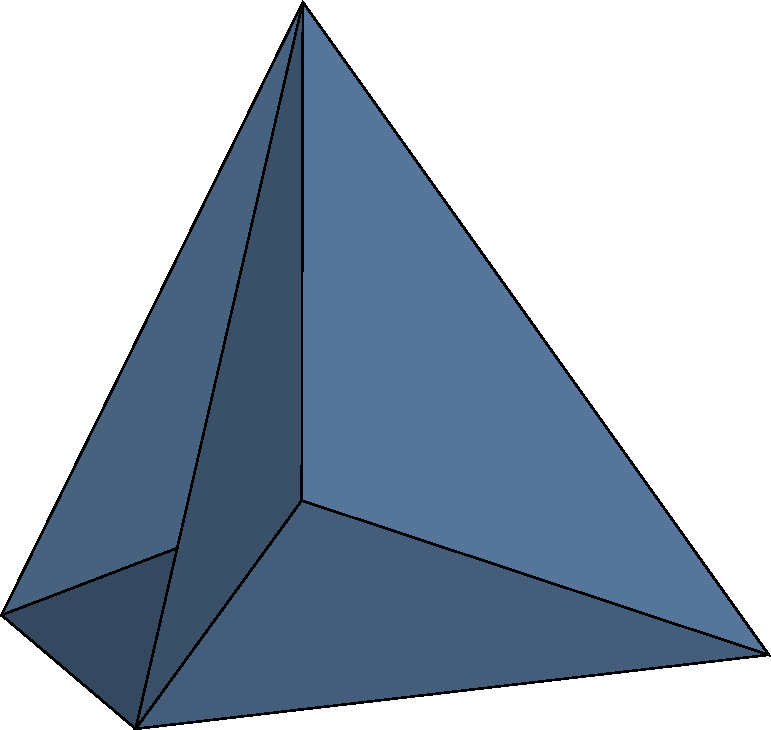
\includegraphics[width=.4\linewidth]{./media/tetra_film.pdf}
\qquad \qquad
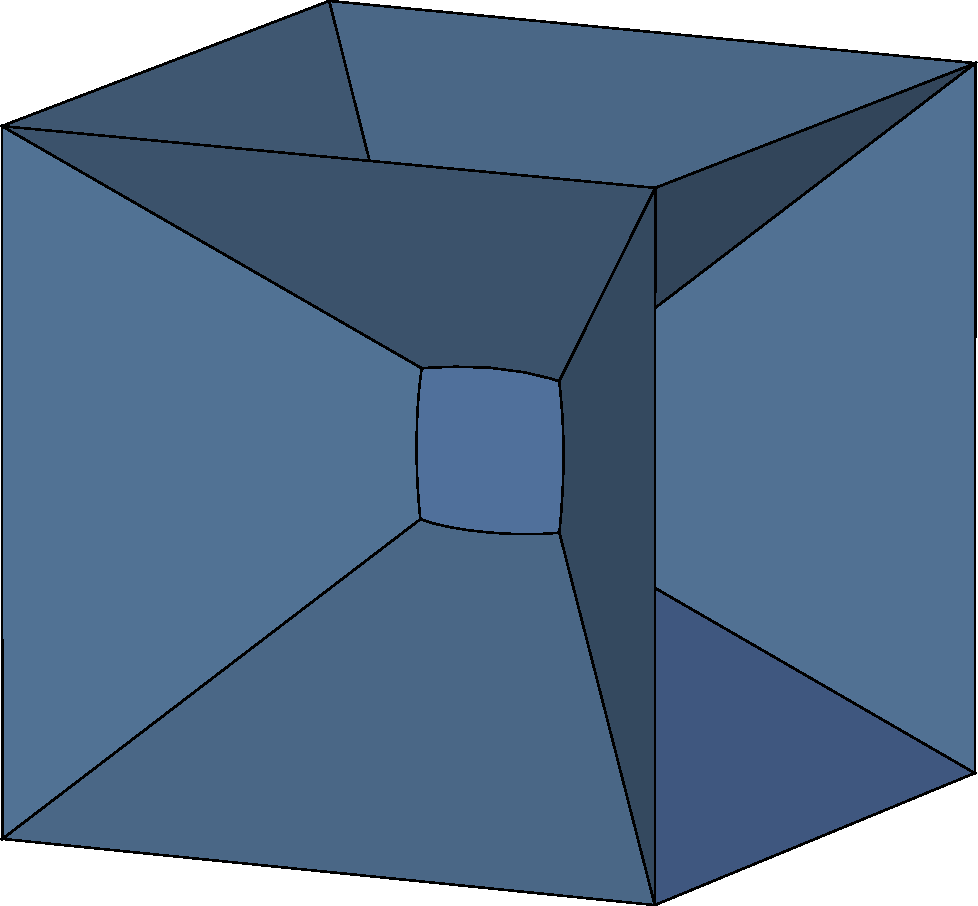
\includegraphics[width=.4\linewidth]{./media/cube_film.pdf}
\end{center}
\end{figure}
\end{frame}

\begin{frame}
\frametitle{Principe}
\begin{itemize}
	\item Une surface est codée par un complexe.
	\item \textit{Evolver} déplace les sommets pour minimiser une énergie. 
% Par exemple: la tension superficielle, l'énergie potentielle gravitationnelle et d'autres. Voir cube.fe, mound.fe
% Descente de gradient
	\item Le déplacements des sommets peut être soumis à des contraintes.
% Par exemple: enfermer une quantité de volume, s'appuyer sur une contrainte et d'autres.
\end{itemize}
\end{frame}

\begin{frame}
\frametitle{Le problème de Plateau}
Inspiré par les films de savon, le \emph{Problème de Plateau} consiste à minimisel l'aire d'une surface s'appuyant sur une frontière.
\begin{figure}[h]
\begin{center}
\includegraphics[width=0.6\linewidth]{./media/soap_film.jpg}
\end{center}
\end{figure}
\end{frame}

\begin{frame}
\frametitle{Quelques limite}
	\begin{itemize}
		\item Pas de frontière glissante..
		\item Il faut que la surface initiale ait la même structure que la surface que l'on veut obtenir.
	\end{itemize}
\end{frame}

\begin{frame}
\frametitle{Imprimer les surfaces}
	\begin{enumerate}
		\item<2-> Exporter le complexe (mesh) au format STL.
		\item<3-> Epaissir la surface avec Blender.
	\end{enumerate}
\end{frame}

\begin{frame}
\begin{center}
\Huge{Fin}\\
\strut\newline
\normalsize{\url{https://github.com/camillelab/evolver}.}
\end{center}
\end{frame}
\end{document}
